\documentclass[8pt,executivepaper]{article}
\usepackage[utf8]{inputenc}
\usepackage[spanish]{babel}
\usepackage{amsmath}
\usepackage{amsfonts}
\usepackage{amssymb}
\usepackage{graphics}
\usepackage{graphicx}
\usepackage[left=1cm,right=1cm,top=2cm,bottom=2cm]{geometry}
\usepackage{imakeidx}
\makeindex[columns=3, title=Alphabetical Index, intoc]
\usepackage{listings}
\usepackage{xcolor}
\usepackage{multicol}
\usepackage{changepage}
\usepackage{float}
\usepackage{cite}
\usepackage{url}
\usepackage{hyperref}
\usepackage{pdfpages}
\usepackage{pgf,pgffor}

\definecolor{codegreen}{rgb}{0,0.6,0}
\definecolor{codegray}{rgb}{0.5,0.5,0.5}
\definecolor{codepurple}{rgb}{0.58,0,0.82}
\definecolor{backcolour}{rgb}{0.95,0.95,0.92}
\lstdefinestyle{mystyle}{
    backgroundcolor=\color{backcolour},
    commentstyle=\color{codegreen},
    keywordstyle=\color{magenta},
    numberstyle=\tiny\color{codegray},
    stringstyle=\color{codepurple},
    basicstyle=\ttfamily\footnotesize,
    breakatwhitespace=false,
    breaklines=true,
    captionpos=b,
    keepspaces=true,
    numbers=left,
    numbersep=5pt,
    showspaces=false,
    showstringspaces=false,
    showtabs=false,
    tabsize=3
}
\lstset{style=mystyle}
\author{González Pardo Adrian}
\date{Mayo 2020}
\title{Reporte de practica 12}
\newcommand\tab[1][1cm]{\hspace*{#1}}
\begin{document}
\maketitle
\section{Código fuente:}
\subsection{Unidad de Control}
\lstinputlisting[language=VHDL]{vhd/unidadControl.vhd}
\subsection{Registro}
\lstinputlisting[language=VHDL]{vhd/registro.vhd}
\subsection{Contador}
\lstinputlisting[language=VHDL]{vhd/contador.vhd}
\subsection{Decodificador}
\lstinputlisting[language=VHDL]{vhd/decodificador.vhd}
\subsection{Mux}
\lstinputlisting[language=VHDL]{vhd/muxD.vhd}
\subsection{Arquitectura completa}
\lstinputlisting[language=VHDL]{vhd/cartaASM.vhd}

\section{Codigo de empaquetado}
\lstinputlisting[language=VHDL]{vhd/paqueteEntidades.vhd}




\section{Test-Bench:}
\subsection{Unidad de Control}
\subsubsection{Codigo}
\lstinputlisting[language=VHDL]{tb/unidadControl_TB.vhd}
\subsubsection{Imagenes}
\begin{center}
  \includegraphics[scale=0.33]{img/unidadControl.png}
\end{center}

\subsection{Registro}
\subsubsection{Codigo}
\lstinputlisting[language=VHDL]{tb/registro_TB.vhd}
\subsubsection{Imagenes}
\begin{center}
  \includegraphics[scale=0.33]{img/registro.png}
\end{center}

\subsection{Contador}
\subsubsection{Codigo}
\lstinputlisting[language=VHDL]{tb/contador_TB.vhd}
\subsubsection{Imagenes}
\begin{center}
  \includegraphics[scale=0.33]{img/contador.png}
\end{center}

\subsection{Decodificador}
\subsubsection{Codigo}
\lstinputlisting[language=VHDL]{tb/decodificador_TB.vhd}
\subsubsection{Imagenes}
\begin{center}
  \includegraphics[scale=0.33]{img/decodificador.png}
\end{center}

\subsection{Mux}
\subsubsection{Codigo}
\lstinputlisting[language=VHDL]{tb/muxD_TB.vhd}
\subsubsection{Imagenes}
\begin{center}
  \includegraphics[scale=0.33]{img/muxD.png}
\end{center}

\subsection{Arquitectura completa}
\subsubsection{Codigo}
\lstinputlisting[language=VHDL]{tb/cartaASM_TB.vhd}
\subsubsection{Imagenes}
\begin{center}
  \includegraphics[scale=0.33]{img/asm-1.png}\\
  \includegraphics[scale=0.33]{img/asm-2.png}\\
  \includegraphics[scale=0.33]{img/asm-3.png}\\
  \includegraphics[scale=0.33]{img/asm-4.png}\\
  \includegraphics[scale=0.33]{img/asm-5.png}
\end{center}

\section{Diagrama RTL}
\subsection{Unidad de Control}
\begin{center}
  \includegraphics[scale=0.7]{rtl/unidadControl.pdf}
\end{center}
\subsection{Registro}
\begin{center}
  \includegraphics[scale=0.7]{rtl/registro.pdf}
\end{center}
\subsection{Contador}
\begin{center}
  \includegraphics[scale=0.7]{rtl/contador.pdf}
\end{center}
\subsection{Decodificador}
\begin{center}
  \includegraphics[scale=0.4]{rtl/decodificador.pdf}
\end{center}
\subsection{Mux}
\begin{center}
  \includegraphics[scale=0.4]{rtl/muxD.pdf}
\end{center}
\subsection{Arquitectura Completa}
\begin{center}
  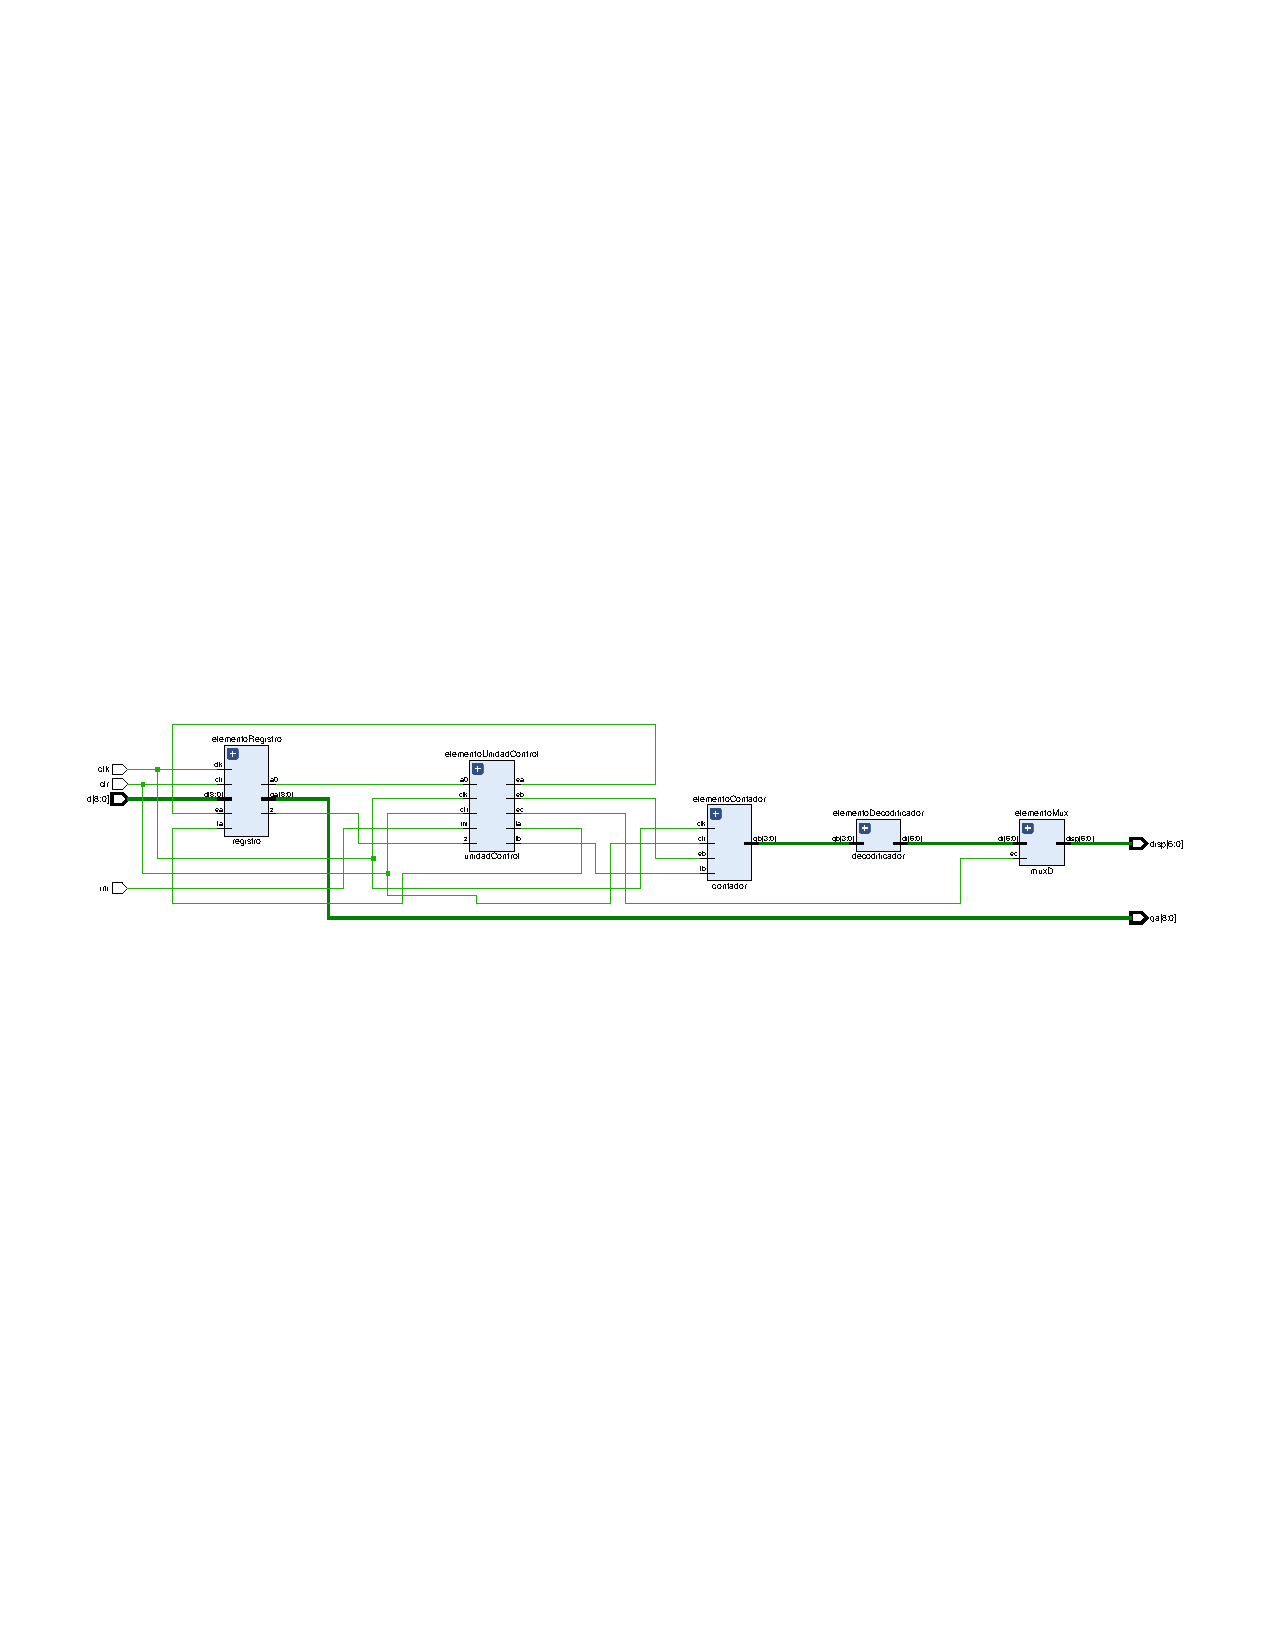
\includegraphics[scale=0.7]{rtl/cartaASM.pdf}
\end{center}
\end{document}
